\documentclass[letterpaper, 10 pt, conference]{ieeeconf}  % Comment this line out if you need a4paper

%\documentclass[a4paper, 10pt, conference]{ieeeconf}      % Use this line for a4 paper

\IEEEoverridecommandlockouts                              % This command is only needed if 
                                                          % you want to use the \thanks command

\overrideIEEEmargins                                      % Needed to meet printer requirements.




% The following packages can be found on http:\\www.ctan.org
\usepackage{graphics} % for pdf, bitmapped graphics files
\usepackage{epsfig} % for postscript graphics files
% \usepackage{times}
% \usepackage{newtxtext,newtxmath} % Times-like text and math fonts

\usepackage{mathptmx} % assumes new font selection scheme installed
\usepackage{times} % assumes new font selection scheme installed
\usepackage{amsmath} % assumes amsmath package installed
\usepackage{amssymb}  % assumes amsmath package installed
% \usepackage[utf8]{inputenc}

\usepackage{cite} % Use cite.sty for numerical citation management
\usepackage[bookmarks=true]{hyperref} % Use hyperref for other links
% \usepackage{hyperref} % Use hyperref for other links
% \usepackage{appendix}

\usepackage{tikz}
\usepackage{float}
\usepackage{svg}
% \usepackage{bm}
\usepackage{balance}

\tikzstyle{block} = [rectangle, minimum width=2cm, minimum height=1cm,text centered, draw=black]
\tikzstyle{block_1} = [rectangle, minimum width=2cm, minimum height=1cm,text centered, draw=black, fill=blue!5]
\tikzstyle{block_2} = [rectangle, minimum width=2cm, minimum height=1cm,text centered, draw=black, fill=red!5]
\tikzstyle{arrow} = [thick,->,>=stealth]
\tikzstyle{arrow_2} = [very thick,->,>=stealth]
\tikzstyle{arrow_3} = [thick,->,>=stealth,dashed]
\tikzstyle{pfr} = [cylinder, draw, minimum height=4cm, minimum width=1cm, shape aspect=1, shape border rotate=180]
\usetikzlibrary{shapes.geometric}


% Override the fake natbib command to allow cite.sty and hyperref to work together
\makeatletter
\let\NAT@parse\undefined
\makeatletter

\title{\LARGE \bf
Model Predictive Control of Axial Dispersion Tubular Reactors\\ with Recycle: Addressing State-delay through Transport PDEs
}


\author{Behrad Moadeli and Stevan Dubljevic$^{1}$% <-this % stops a space
\thanks{$^{1}$Behrad Moadeli and Stevan Dubljevic are with the Department of Chemical and Materials Engineering,
University of Alberta, Edmonton, AB, Canada T6G 1H9
{\tt\small moadeli@ualberta.ca}, {\tt\small stevan.dubljevic@ualberta.ca}}%
\thanks{Funding provided by the Natural Sciences and Engineering Research Council of Canada—NSERC (RGPIN-2022-03486).}% <-this % stops a space
}


\begin{document}



\maketitle
\thispagestyle{empty}
\pagestyle{empty}


%%%%%%%%%%%%%%%%%%%%%%%%%%%%%%%%%%%%%%%%%%%%%%%%%%%%%%%%%%%%%%%%%%%%%%%%%%%%%%%%
\begin{abstract}

        This paper presents the model predictive control of an axial tubular reactor with a recycle stream, where the intrinsic time delay imposed by the recycle stream—often overlooked in chemical engineering process control studies—is modeled as a transport PDE. This leads to a boundary-controlled system of coupled parabolic and hyperbolic PDEs under Danckwerts boundary conditions, specific for this reactor type. A discrete-time linear model predictive controller is designed to stabilize the system. Utilizing Caley-Tustin time discretization along with the late lumping approach, the system's infinite-dimensional characteristics are preserved with no need for model reduction or spatial approximation. Numerical simulations demonstrate the controller's effectiveness in stabilizing an unstable system while satisfying input constraints.

\end{abstract}

\section{Introduction}

Many processes in the chemical and petrochemical sectors involve states that evolve over space and time, commonly represented by partial differential equations (PDEs) as distributed parameter systems (DPS) \cite{ray1981advanced}. 
The infinite-dimensional nature of DPSs presents specific challenges in control and estimation, making this a prominent area of research. Two main methods are often applied to control DPSs: \textit{Early Lumping} and \textit{Late Lumping}. 
Early Lumping reduces the system to a finite-dimensional approximation through spatial discretization early in the modeling stage, allowing for the application of standard control techniques \cite{davison1976robust}. 
However, this method can lead to inaccuracies due to mismatches between the reduced model and the original system dynamics \cite{moghadam2012infinite}. 
Late Lumping, by contrast, preserves the system's infinite-dimensional structure until the final stages of controller implementation, resulting in a control approach that is more complex but achieves greater fidelity to the original dynamics.

A range of studies in chemical engineering have applied the late lumping method to control infinite-dimensional systems, specifically targeting convection-reaction processes governed by first-order hyperbolic PDEs and diffusion-convection-reaction processes described by second-order parabolic PDEs. 
In \cite{christofides1996feedback}, the robust control of first-order hyperbolic PDEs is explored, demonstrating the stabilization of a plug flow reactor system using a distributed input. 
A boundary feedback stabilization approach using the backstepping method is presented in \cite{krstic2008backstepping} for a comparable system of first-order hyperbolic PDEs. 
The work in \cite{xu2016state} introduces a state feedback regulator design for a countercurrent heat exchanger system, providing another example of a chemical engineering DPS governed by first-order hyperbolic PDEs, distinct from tubular reaction systems. 
Highlighting the role of dispersion in axial dispersion tubular reactors, \cite{christofides1998robust} examines the robust control of diffusion-convection-reaction systems governed by second-order parabolic PDEs. 
In \cite{dubljevic2006predictive2}, a late-lumping approach is employed to develop a low-dimensional predictive controller for a diffusion-convection-reaction system, utilizing modal decomposition to capture the system's dominant modes. 
A similar method is applied in \cite{khatibi2021model} to design an observer-based model predictive controller (MPC) for an axial dispersion tubular reactor, accounting for the impact of recycle streams, a common feature in industrial chemical reactors. 
Different aspects of state reconstruction for DPSs are addressed in several works where the design of a discrete-time Luenberger observer is adressed for the class of DPSs, where no spatial discretization is required; a key feature of the late lumping approach  \cite{dochain2000state, dochain2001state, alonso2004optimal, ali2015review}.

In addition to dynamic systems distributed over space, dynamic systems that exhibit time delays are also classified as DPSs \cite{curtainbook}. 
In the field of control theory for infinite-dimensional systems, delay systems are either represented as delay differential equations (DDEs) or as transport PDEs, with the latter being advantageous in more complex scenarios, e.g. in the presence of spatial dynamics \cite{krstic2009book}. 
When it comes to chemical engineering applications of control theory, delays are often introduced as the result of input or output delays, while state delays are less frequently addressed in the literature; most probably since not many applications in this field can be described by state delays, in contrast with other domains of control theory, such as signal processing or mechanical systems. 
Input/output delays are generally handled by introducing a transportation lag block at either the input or output of the system, leading to a cascade PDE system \cite{Hiratsuka1969IEEE, mohammadi2012lq, Guilherme2019ACC}. 
In one of the few studies addressing state delays in this area, \cite{ozorio2019heat} investigates a delayed-state distributed parameter system where a full-state and output feedback regulator is designed for a heat exchanger system. 
Here, the state delay arises from the time taken for a stream to exit one pass of the heat exchanger and enter the next. 
Similarly, in \cite{qi2021output}, a tubular reactor system is considered, where state delay is introduced by the recycle delay in the system, without accounting for the diffusion term along the reactor. 
Even in \cite{khatibi2021model}, where a recycle stream is incorporated for a distributed diffusion-convection-reaction system, the recycle is assumed to be instantaneous—an assumption that creates a gap in the literature on diffusion-convection-reaction systems with recycle streams that impose a state delay.

In this work, an axial dispersion tubular reactor equipped with recycle is addressed as a diffusion-convection-reaction DPS. First, the reactor is modeled by a second order parabolic PDE, where the recycle stream poses a state delay, resulting in a first order hyperbolic transport PDE. 
Therefore, a system of coupled hyperbolic and parabolic PDEs is obtained to describe the infinite-dimensional model of the plant. 
The resolvent operator of the system is then obtained in an exact closed form, omitting the need for spatial discretization following the late lumping approach. 
The continous-time system is then discrtetized to enable the implementation of MPC as a digital controller. This is done using Caley-Tustin time discretization technique, i.e. a Crank-Nicolson type of discretization that preserves the conservative characteristics of the continuous system, mitigating the need for model reduction \cite{havu2007cayley, xu2017linear}. 
An infinite-dimensional Luenberger observer is also designed to reconstruct the states of the system, addressing the controller's limited access to system's full-state. 
As a result, through numerical simulations, the observer-based output feedback MPC is shown to successfully stabilize a system while adhering to input constraints, despite the original system being unstable.
\section{Methodology}

\subsection{Model representation}

The chemical process depicted in Fig.~\ref{fig:reactor_scheme} illustrates a first-order irreversible chemical reaction within an axial dispersion tubular reactor \cite{levenspiel1998chemical}. The reactor features a recycle mechanism, allowing a portion of the product stream to re-enter the reactor, ensuring the consumption of any unreacted substrate. The reactor's dynamics can be described by a second-order parabolic PDE, a common class of equations used to characterize diffusion-convection-reaction systems \cite{jensen1982bifurcation}. The resulting PDE that describes the reactor model is given by \eqref{eq:PDE_original_model}, subject to the boundary conditions in \eqref{eq:BC}, obtained by utilizing first-principle modeling through relevant mass balance relations on an infinitesimally thin disk element along the longitudinal axis of the reactor.

\begin{figure}[!htbp] 
    \centering
    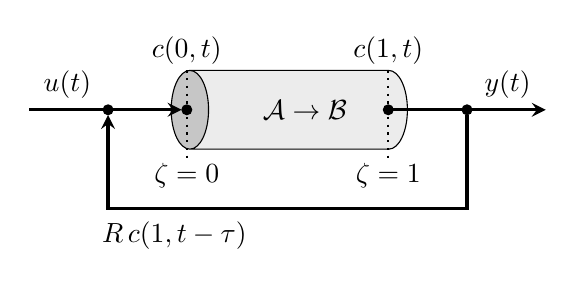
\begin{tikzpicture}
        \node (pfr) [cylinder, draw, minimum height=3cm, minimum width=1cm, shape aspect=1, shape border rotate=180, cylinder uses custom fill, cylinder end fill=gray!45, cylinder body fill=gray!15] {$\mathcal{A} \rightarrow \mathcal{B}$};
        \node (pfr_inlet) [circle, left of=pfr, xshift=-0.5cm, fill=black, draw, inner sep=0pt, minimum size=0.25cm, scale=0.5] {};
        \node (pfr_outlet) [circle, at={(pfr.east)}, shift={(-0.25cm,0)}, fill=black, draw, inner sep=0pt, minimum size=0.25cm, scale=0.5] {};
        \node (recycle_right) [circle, right of=pfr_outlet, fill=black, draw, inner sep=0pt, minimum size=0.25cm, scale=0.5] {};
        \node (recycle_left) [circle, left of=pfr_inlet, fill=black, draw, inner sep=0pt, minimum size=0.25cm, scale=0.5] {};
        
        \draw[dotted, thick] ([yshift=0.5cm]pfr_inlet.center) -- node[at end, below, yshift=0.1cm] {$\zeta = 0$} ([yshift=-0.65cm]pfr_inlet.center);
        \draw[dotted, thick] ([yshift=0.5cm]pfr_outlet.center) -- node[at end, below, yshift=0.1cm] {$\zeta = 1$} ([yshift=-0.65cm]pfr_outlet.center);
        
        \node[below of=recycle_left, node distance=1.3cm, anchor=north west, xshift=-0.2cm] {$R \, c(1, t-\tau)$};
        \node[above of=pfr_inlet, node distance=0.75cm,] {$c(0, t)$};
        \node[above of=pfr_outlet, node distance=0.75cm,] {$c(1, t)$};
        
        \draw [arrow_2] (pfr_outlet) -- node[near end, above] {$y(t)$} ++(2,0);
        \draw [arrow_2] (pfr_inlet) ++(-2,0) coordinate(start) -- node[near start, above] {$u(t)$} (pfr_inlet);
        \draw [arrow_2] (recycle_right) -- ++(0,-1.25) -| (recycle_left);
        
    \end{tikzpicture}
    \caption{Axial tubular reactor with recycle stream.}
    \label{fig:reactor_scheme}
    % \pdfbookmark[2]{Figure: Reactor Scheme}{fig:reactor_scheme}
\end{figure}

\begin{equation} \label{eq:PDE_original_model}
    \dot{c}(\zeta, t) = D \partial_{\zeta \zeta} c(\zeta, t) - v \partial_\zeta c(\zeta, t) + k_r c(\zeta, t)
\end{equation}

\begin{align} \label{eq:BC}
    \begin{cases}
        &D \partial_\zeta c(0, t) - v c(0, t) = -v \left[ R c(1, t-\tau) + (1-R) u(t) \right] \\
        &\partial_\zeta c(1, t) = 0 \\
        &y(t) = c(1, t)
    \end{cases}
\end{align}

Here, $c(\zeta, t)$ is the concentration of the product along the reactor, representing the state of the system. The physical parameters $D$, $v$, $k_r$, $R$, and $\tau$ represent the diffusion coefficient, flow velocity along the reactor, reaction constant, recycle ratio, and residence time of the recycle flow, respectively. The coordinate system in space and time is represented by $\zeta$ and $t$, where $\zeta \in [0, 1]$ and $t \in [0, \infty)$.

In an attempt to make the model more realistic for common axial dispersion tubular reactors in chemical industry, Dankwerts boundary conditions are chosen as they are known to be suitable for this purpose by accounting for deviations from perfect mixing and piston flow, assuming negligible transport lags in connecting lines \cite{danckwerts1993continuous}. The delayed state resulting from the recycled portion of the flow, occurring $\tau$ seconds back in time, is applied at the inlet boundary condition, as shown in \eqref{eq:BC}.

In the case where the problem involves similar forms of PDEs, an effective general practice to address delays in systems is to reformulate the problem such that the notion of delay is replaced with an alternative transport PDE. Therefore, a new state variable $\underline{x}(\zeta, t) \equiv [x_1(\zeta, t), x_2(\zeta, t)]^T$ is defined as a vector of functions, where $x_1(\zeta, t)$ represents the concentration within the reactor—analogous to $c(\zeta,t)$—and $x_2(\zeta, t)$ is introduced as a new state variable to account for the concentration along the recycle stream. The delay is thus modeled as a pure transport process, wherein the first state $x_1(\zeta, t)$ is transported from the reactor outlet to the inlet, experiencing a delay of $\tau$ time units while in the recycle stream. This makes all state variables expressed explicitly at a specific time instance $t$, resulting in the standard state-space form for a given infinite-dimensional linear time-invariant (LTI) system $\dot{\underline{x}} = \mathfrak{A} \underline{x} + \mathfrak{B} u$. Here, $\mathfrak{A}$ is a linear operator $\mathcal{L}(X)$ acting on a Hilbert space $X: L^2[0,1] \times L^2[0,1]$ and $\underline{x}(\zeta,t)$, as defined previously, is the vector of functions describing the states of the system. The operator $\mathfrak{A}$ and its domain are defined in detail as shown in \eqref{eq:operator_A}. Also, $\mathfrak{B}$ is a linear operator that maps the scalar input from input-space onto the state space, as defined in \eqref{eq:operator_B}.

\begin{equation} \label{eq:operator_A}
    \begin{aligned}
        \mathfrak{A} \equiv&
        \begin{bmatrix}
            D \partial_{\zeta \zeta} - v \partial_\zeta + k_r & 0 \\
            0 & \frac{1}{\tau} \partial_\zeta
        \end{bmatrix}\\
        D(\mathfrak{A}) =& \Bigl\{ \underline{x}(\zeta) = [x_1(\zeta), x_2(\zeta)]^T \in X:\\
        &\underline{x}(\zeta), \partial_\zeta \underline{x}(\zeta), \partial_{\zeta \zeta} \underline{x}(\zeta) \quad \mathrm{a.c.},\\
        &D \partial_\zeta x_1(0) - v x_1(0) = -v R x_2(0),\\
        &\partial_\zeta x_1(1) = 0,
        x_1(1) = x_2(1) \Bigr\}
    \end{aligned}
\end{equation}

\begin{equation} \label{eq:operator_B}
    \begin{aligned}
        \mathfrak{B} &\equiv
        \begin{bmatrix}
            \delta(\zeta) \\
            0
        \end{bmatrix} v (1-R) \\
        D(\mathfrak{B}) &= \Bigl\{ u \in \mathbb{R} \Bigr\}
    \end{aligned}
\end{equation}

where $\delta(\zeta)$ is dirac delta function. This will enable the derivation of the system's spectrum using the eigenvalue problem. The characteristics equation of the system is obtained by solving the equation $det(\mathfrak{A}-\lambda_i~I)~=~0$ for $\lambda_i$, where $\lambda_i \in \mathbb{C}$ is the $i^{\text{th}}$ eigenvalue of the system and $I$ is the identity operator. Attempts to analytically solve this equation has failed; therefore, it is solved numerically using the parameters in Table~\ref{tab:pars}. The resulting eigenvalue distribution is depicted in Figure~\ref{fig:eigval_dist} in the complex plane.

\begin{figure}[!htbp]
    \centering
    \includesvg[inkscapelatex=false, width=0.35\textwidth, keepaspectratio]{Figures/eig_val_dist_R_0.3.svg}
    \caption{Eigenvalues of operator $\mathfrak{A}$.}
    \label{fig:eigval_dist}
\end{figure}


\begin{table}[ht]
    \centering
    \caption{Physical Parameters for the System}
    \label{tab:pars}
    \begin{tabular}{|c|c|c|c|}
    \hline
    \textbf{Parameter}        & \textbf{Symbol} & \textbf{Value}     & \textbf{Unit}    \\ \hline
    Diffusivity               & $D$             & $2\times10^{-5}$   & ${m^2}/{s}$      \\ \hline
    Velocity                  & $v$             & $0.01$   & ${m}/{s}$        \\ \hline
    Reaction Constant         & $k_r$           & $1.5$              & $s^{-1}$         \\ \hline
    Recycle Residence Time    & $\tau$          & $80$               & $s$              \\ \hline
    Recycle Ratio             & $R$             & $0.3$              & $-$              \\ \hline
    \end{tabular}
\end{table}

\subsection{Adjoint system}

Next step is to obtain the adjoint system operators $\mathfrak{A}^*$ and $\mathfrak{B}^*$. Utilizing the relation $\langle \mathfrak{A} \underline{x} + \mathfrak{B} u, \underline{y}\rangle = \langle \underline{x}, \mathfrak{A}^* \underline{y}\rangle + \langle u, \mathfrak{B}^* \underline{y}\rangle$, the adjoint operators $\mathfrak{A}^*$ and $\mathfrak{B}^*$ are obtained as shown in \eqref{eq:adjoint_A} and \eqref{eq:adjoint_B}, respectively.


\begin{equation} \label{eq:adjoint_A}
    \begin{aligned}
        {\mathfrak{A}}^{*} =&
        \begin{bmatrix}
            D \partial_{\zeta \zeta} + v \partial_\zeta +k_r & 0\\
            0 & -\frac{1}{\tau} \partial_\zeta
        \end{bmatrix}\\
        D(\mathfrak{A}^*) =& \Bigl\{ \underline{y} = [y_1, y_2]^T \in Y:\\
        &\underline{y}(\zeta), \partial_\zeta \underline{y}(\zeta), \partial_{\zeta \zeta} \underline{y}(\zeta) \quad \mathrm{a.c.},\\
        &D \partial_\zeta y_1(1) + v y_1(1) = \frac{1}{\tau} y_2(1), \\
        &R v y_1(0) = \frac{1}{\tau} y_2(0), 
        \partial_\zeta y_1(0) = 0 \Bigr\}
    \end{aligned}
\end{equation}

\begin{equation} \label{eq:adjoint_B}
    \mathfrak{B}^* (\cdot) = \Bigl[ v(1-R) \int_0^1 \delta(\zeta) (\cdot) d\zeta \quad , \quad 0 \Bigr]
\end{equation}

Once the adjoint operators are determined, the eigenfunctions $\{ \underline{\phi_i}(\zeta), \underline{\psi_i}(\zeta) \}$ (for $\mathfrak{A}$ and $\mathfrak{A}^*$, respectively) may be obtained and properly scaled following the calculation of eigenvalues. The set of scaled eigenfunctions will then form a bi-orthonormal basis for the Hilbert space $X$; which will be later used in the controller design. It is important to note that the system is not self adjoint, as the obtained adjoint operator and its domain are not the same as the original operator and its domain.

\subsection{Resolvent operator}

One must obtain the resolvent operator of the system $\mathfrak{R}(s, \mathfrak{A}) = (sI-\mathfrak{A})^{-1}$ prior to constructing the discrete-time representation of the system. One way to obtain it is by utilizing the modal characteristics of the system, resulting in an infinite-sum representation of the operator. While being a common practice in the literature, truncating the infinite-sum representation for numerical implementation may lead to a loss of accuracy. Another way to express the resolvent operator is by treating it as an operator that maps either the initial condition of the system $\underline{x}(\zeta,0)$ or the input $u(t)$, to the Laplace transform of the state of the system $\underline{X}(\zeta, s)$. This approach, although more computationally intensive, results in a closed form expression for the resolvent operator, preserving the infinite-dimensional nature of the system. In \eqref{eq:resolvent}, Laplace transform is applied to the LTI representation of the system for both zero-input response and zero-state response to obtain a general expression for the resolvent operator.

\begin{equation} \label{eq:resolvent}
    \begin{aligned}
        \dot{\underline{x}}(\zeta, t) &= \mathfrak{A} \underline{x}(\zeta, t) + \mathfrak{B} u(t) \xrightarrow{\mathcal{L}}\\
        s \underline{X}(\zeta,s) - \underline{x}(\zeta,0) &= \mathfrak{A} \underline{X}(\zeta,s) + \mathfrak{B} U(s)\\
        &\hspace{-7.5em}\begin{cases}
            \xrightarrow{u = 0} &\underline{X}(\zeta,s) = (sI - \mathfrak{A})^{-1} \underline{x}(\zeta,0) = \mathfrak{R}(s, \mathfrak{A}) \underline{x}(\zeta,0)\\
            \xrightarrow{\underline{x}(0, \zeta)}& \underline{X}(\zeta,s) = (sI - \mathfrak{A})^{-1} \mathfrak{B} U(s) = \mathfrak{R}(s, \mathfrak{A}) \mathfrak{B} U(s)
        \end{cases}
    \end{aligned}
    \end{equation}
    
    The goal is to obtain the solution for $\underline{X}(\zeta, s)$ and compare it with the general expression obtained in \eqref{eq:resolvent} to get the closed form expression for the resolvent operator. First step is to apply Laplace transform to the original system of PDEs in \eqref{eq:operator_A}. The second order derivative term is decomposed to two first order PDEs, constructing a new $3 \times 3$ system of first order ODEs with respect to $\zeta$ after Laplace transformation, as shown in \eqref{eq:laplace_transformed}.
    
    \begin{equation} \label{eq:laplace_transformed}
    \begin{aligned}
        \partial_\zeta \overbrace{\begin{bmatrix}
            X_1(\zeta,s)\\ \partial_\zeta X_1(\zeta,s)\\ X_2(\zeta,s)
        \end{bmatrix}}^{\underline{\tilde{X}}(\zeta,s)} &= \overbrace{\begin{bmatrix}
            0 & 1 & 0\\
            \frac{s-k}{D} & \frac{v}{D} & 0\\
            0 & 0 & s\tau
            \end{bmatrix}}^{P(s)} \, \begin{bmatrix}
                X_1(\zeta,s)\\ \partial_\zeta X_1(\zeta,s)\\ X_2(\zeta,s)
            \end{bmatrix} \\
            &+ \underbrace{\begin{bmatrix}
                0\\ -\frac{x_1(\zeta,0)}{D} + v(1-R) \delta(\zeta) U(s)\\ -\tau x_2(\zeta,0)
            \end{bmatrix}}_{Z(\zeta,s)} \\
            \Rightarrow \partial_\zeta \underline{\tilde{X}}(\zeta,s) &= P(s) \underline{\tilde{X}}(\zeta,s) + Z(\zeta,s)
    \end{aligned}
    \end{equation} 
    
    with solution given by \eqref{eq:ODE_solution}.
    
    \begin{equation} \label{eq:ODE_solution}
        \underline{\tilde{X}}(\zeta,s) = \underbrace{e^{P(s)\zeta}}_{T(\zeta,s)} \underline{\tilde{X}}(0,s) + \int_0^\zeta \underbrace{e^{P(s)(\zeta - \eta)}}_{F(\zeta, \eta)} Z(\eta,s) d\eta
    \end{equation}
    
    Since the boundary conditions are not homogeneous, $\underline{\tilde{X}}(0,s)$ needs to be obtained by solving the system of algebraic equations given in \eqref{eq:BC_AE}; which is the result of applying Danckwerts boundary conditions to the Laplace transformed system of PDEs at $\zeta = 1$.
    
    \begin{equation} \label{eq:BC_AE}
    \begin{aligned}
            &\overbrace{\begin{bmatrix}
                -v & D & Rv\\
                T_{11}(1,s) & T_{12}(1,s) & -T_{33}(1,s)\\
                T_{21}(1,s) & T_{22}(1,s) & 0
            \end{bmatrix}}^{M^{-1}(s)} \underline{\tilde{X}}(0,s) =\\ 
            &\underbrace{\int_0^1 \begin{bmatrix}
                0\\ F_{33}(1, \eta) Z_3(\eta,s) - F_{12}(1, \eta) Z_2(\eta,s)\\ -F_{22}(1, \eta) Z_2(\eta,s)
            \end{bmatrix} d\eta}_{\underline{b}(s)} \\
            \Rightarrow &\underline{\tilde{X}}(0,s) = M(s) \underline{b}(s)
    \end{aligned}
    \end{equation}
    
    Having access to $\underline{\tilde{X}}(0,s)$, the solution for $\underline{X}(\zeta,s)$ can be explicitly derived. The resolvent operator for zero-input and zero-state cases are therefore obtained in a closed form as shown in \eqref{eq:resolvent_x} and \eqref{eq:resolvent_u}, respectively.
    
    \begin{equation} \label{eq:resolvent_x}
    \begin{aligned}
        &U(s) = 0 \Rightarrow \mathfrak{R}(s, \mathfrak{A}) \underline{(\cdot)} = \begin{bmatrix}
            \mathfrak{R}_{11} & \mathfrak{R}_{12}\\
            \mathfrak{R}_{21} & \mathfrak{R}_{22}
        \end{bmatrix} \begin{bmatrix}
            (\cdot)_1\\ (\cdot)_2
        \end{bmatrix} \Rightarrow\\
        &\mathfrak{R}_{11} = \sum_{j=1}^2 \frac{T_{1j}(\zeta)}{D} \int_0^1 \left[ M_{j2} F_{12}(1,\eta) + M_{j3} F_{22}(1,\eta) \right] (\cdot)_1 d\eta\\
        &\hspace{2.5em} -\frac{1}{D} \int_0^{\zeta} F_{12}(\zeta, \eta) (\cdot)_1 d\eta\\
        &\mathfrak{R}_{12} = \sum_{j=1}^2 -\tau T_{1j}(\zeta) \int_0^1 M_{j2} F_{33}(1,\eta) (\cdot)_2 d\eta\\
        &\mathfrak{R}_{21} = \frac{T_{33}(\zeta)}{D} \int_0^1 \left[ M_{32} F_{12}(1,\eta) + M_{33} F_{22}(1,\eta) \right] (\cdot)_1 d\eta\\
        &\mathfrak{R}_{22} = -\tau T_{33}(\zeta) \int_0^1 M_{32} F_{33}(1,\eta) (\cdot)_2 d\eta\\
        &\hspace{2.5em} -\tau \int_0^{\zeta} F_{33}(\zeta, \eta) (\cdot)_2 d\eta
    \end{aligned}
    \end{equation}
    
    \begin{equation} \label{eq:resolvent_u}
    \begin{aligned}
        &\underline{x}(\zeta,0) = 0 \Rightarrow \mathfrak{R}(s, \mathfrak{A}) \mathfrak{B} (\cdot) = \begin{bmatrix}
            \mathfrak{R}_{1} \mathfrak{B}\\
            \mathfrak{R}_{2} \mathfrak{B}
        \end{bmatrix} (\cdot) \Rightarrow\\
        &\mathfrak{R}_{1} \mathfrak{B} = -v(1-R) \bigl[ \sum_{j=1}^{2} T_{1j}(\zeta) (M_{j2} T_{12}(1) + M_{j3} T_{22}(1)) \\
        &\hspace{3em} - T_{12}(\zeta) \bigr] (\cdot)\\
        &\mathfrak{R}_{2} \mathfrak{B} = -v(1-R) \left[ T_{33}(\zeta) (M_{32} T_{12}(1) + M_{33} T_{22}(1)) \right] (\cdot)
    \end{aligned}
    \end{equation}

Since the system generator $\mathfrak{A}$ is not self-adjoint, the resolvent operator for the adjoint system shall also be obtained. This is done in a similar manner as the original system, resulting in a closed-form expression for the adjoint resolvent operator $\mathfrak{R}^*(s, \mathfrak{A}^*)$. To avoid redundancy, the derivation of the resolvent operator for the adjoint system is not included in this manuscript.

\subsection{Caley-Tustin time discretization}

Having access to the resolvent operators of the original and the adjoint system, the Caley-Tustin time-discretization may be utilized to map the continuous-time setting to the discrete-time setting without losing crucial dynamical properties of the system, such as stability and controllability. This Crank-Nicolson type of discretization is also known as the lowest order symplectic integrator in Gauss quadrature-based Runge-Kutta methods \cite{hairer2006geometric}. Considering $\Delta t$ as the sampling time, and assuming a piecewise constant input within time intervals (a.k.a. zero-order hold), the discrete-time representation $\underline{x}(\zeta, k) = \mathfrak{A}_d \underline{x}(\zeta, k-1) + \mathfrak{B}_d u(k)$ is obtained, with discrete-time operators $\mathfrak{A}_d$ and $\mathfrak{B}_d$ defined in \eqref{eq:discrete_AB}, where $\alpha = 2/{\Delta t}$.

\begin{equation} \label{eq:discrete_AB}
    \begin{bmatrix}
        \mathfrak{A}_d & \mathfrak{B}_d
    \end{bmatrix} = 
    \begin{bmatrix}
        -I + 2\alpha \mathfrak{R}(\alpha, \mathfrak{A}) & \sqrt{2\alpha} \mathfrak{R}(\alpha, \mathfrak{A}) \mathfrak{B}
    \end{bmatrix}
\end{equation}

As required for systems with nonself-adjoint generators, the adjoint discrete-time operators $\mathfrak{A}_d^*$ and $\mathfrak{B}_d^*$ are also obtained in a similar manner, as shown in \eqref{eq:discrete_AB_star}.

\begin{equation} \label{eq:discrete_AB_star}
    \begin{bmatrix}
        \mathfrak{A}_d^* & \mathfrak{B}_d^*
    \end{bmatrix} = 
    \begin{bmatrix}
        -I + 2\alpha \mathfrak{R}^*(\alpha, \mathfrak{A}^*) & \sqrt{2\alpha} \mathfrak{B}^* \mathfrak{R}^*(\alpha, \mathfrak{A}^*)
    \end{bmatrix}
\end{equation}

\subsection{Model predictive control design}

The proposed MPC, as shown in Fig.~\ref{fig:block_diagram}, is developed in this section with the goal of stabilizing the given unstable infinite-dimensional system within an optimal framework while satisfying input constraints. An infinite-time open-loop objective function sets the foundation of the controller design in the discrete-time setting at each sampling instant $k$, which consists of a weighted sum of state deviations and actuation costs for all future time instances, subject to the system dynamics and input constraints, as shown in \eqref{eq:MPC_inf_time}.

\begin{figure}[!htbp]
    \centering
    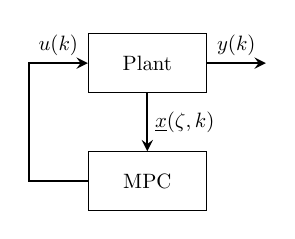
\begin{tikzpicture}[node distance=2cm, scale=0.75, transform shape]
        \node (plant) [block] {Plant};
        \node (MPC) [block, below of=plant] {MPC};
        \draw [arrow] (plant.south) -- node[midway, right] {$\underline{x}(\zeta,k)$} (MPC.north);
        \draw [arrow] (MPC.west) -- ++(-1,0) |- node[near end, above] {$u(k)$} (plant.west);
        \draw [arrow] (plant.east) -- node[midway, above] {$y(k)$} ++(1,0);
    \end{tikzpicture}
    \caption{Proposed full-state feedback model predictive control system.}
    \label{fig:block_diagram}
\end{figure}

\begin{equation} \label{eq:MPC_inf_time}
    \begin{aligned}
        \min_{U} \quad \sum_{l=0}^{\infty} &\langle \underline{x}(\zeta, k+l | k), \mathfrak{Q} \underline{x}(\zeta, k+l | k) \rangle \\
        + &\langle u(k+l+1 | k), \mathfrak{F} u(k+l+1|k) \rangle \\
        \, \\
        \text{s.t.} \quad &\underline{x}(\zeta, k+l | k) = \mathfrak{A}_d \underline{x}(\zeta, k+l-1 | k) + \mathfrak{B}_d u(k+l | k) \\
        &u^{min} \leq u(k+l | k) \leq u^{max}
    \end{aligned}
\end{equation}

where $\mathfrak{Q}$ and $\mathfrak{F}$ are positive definite operators of appropriate dimensions, responsible for penalizing state deviations and actuation costs, respectively. The notation $(k+l|k)$ indicates the future time states or input instance $k+l$ obtained at time $k$. The infinite-time optimization problem may be reduced to a finite-time setup by assigning zero-input beyond a certain control horizon $N$, resulting in the optimization problem in \eqref{eq:MPC_finite_time}.

\begin{equation} \label{eq:MPC_finite_time}
    \begin{aligned}
        \min_{U} \quad \sum_{l=0}^{N-1} &\langle \underline{x}(\zeta, k+l | k), \mathfrak{Q} \underline{x}(\zeta, k+l | k) \rangle \\
        + &\langle u(k+l+1 | k), \mathfrak{F} u(k+l+1|k) \rangle \\
        + &\langle \underline{x}(\zeta, k+N | k), \mathfrak{P} \underline{x}(\zeta, k+N | k) \rangle \\
        \, \\
        \text{s.t.} \quad &\underline{x}(\zeta, k+l | k) = \mathfrak{A}_d \underline{x}(\zeta, k+l-1 | k) + \mathfrak{B}_d u(k+l | k) \\
        &u^{min} \leq u(k+l | k) \leq u^{max} \\
        & \langle \underline{x}(\zeta, k+N | k), \underline{\phi_u}(\zeta) \rangle = 0
    \end{aligned}
\end{equation}

Obtained as the solution to the discrete-time Lyapunov equation, $\mathfrak{P}$ is the terminal cost operator as shown in \eqref{eq:terminal_cost}; which can be proven to be positive definite only if the terminal state $\underline{x}(\zeta, k+N | k)$ is in a stable subspace. Therefore, an equality constraint is introduced to guarantee that the resulting quadratic optimization problem is convex. The terminal constraint is enforced by setting the projection of the terminal state onto the unstable subspace of the system to zero \cite{curtainbook, xu2017linear, khatibi2021model}. Here, $\underline{\phi_u}(\zeta)$ is the set of unstable eigenfunctions of the system, for all eigenvalues where $\operatorname{Re}(\lambda_u) \geq 0$.

\begin{equation} \label{eq:terminal_cost}
    \mathfrak{P} (\cdot) = \sum_{m=0}^{\infty} \sum_{n=0}^{\infty} 
    -\frac{
        \langle \underline{\phi_m} , \mathfrak{Q} \underline{\psi_n} \rangle
    }{
        \lambda_m + \overline{\lambda_n}
    }
    \langle (\cdot) , \underline{\psi_n} \rangle \phi_m
\end{equation}

One may further process the optimization problem in \eqref{eq:MPC_finite_time} to obtain a standard format for quadratic programming (QP) solvers by substituting the future states in terms of the current state and the sequence of future inputs using system dynamics expression. The resulting QP problem is given in \eqref{eq:MPC_QP}. The optimal input sequence $U$ is then obtained by solving the QP problem at each sampling instant $k$. To implement a receding horizon control strategy, only the first input of the optimal sequence $u(k+1|k)$ is applied to the system, and the optimization problem is solved again at the next sampling instant $k+1$.

\begin{equation} \label{eq:MPC_QP}
    \begin{aligned}
        \min_{U} &J = U^T \langle I,H \rangle U + 2U^T \langle I, P \underline{x}(\zeta, k|k) \rangle \\
        \text{s.t.} &\qquad U^{min} \leq U \leq U^{max} \\
        &\qquad T_u \underline{x}(\zeta, k|k) + S_u U = 0
        \, \\
        \text{with } &H = \\
        &\hspace{-3.5em }\begin{bmatrix}
            \mathfrak{B}_d^* \mathfrak{P} \mathfrak{B}_d + \mathfrak{F} & \mathfrak{B}_d^* \mathfrak{A}_d^* \mathfrak{P} \mathfrak{B}_d & \cdots &  \mathfrak{B}_d^* {\mathfrak{A}_d^*}^{N-1} \mathfrak{P} \mathfrak{B}_d \\
            \mathfrak{B}_d^* \mathfrak{P} \mathfrak{A}_d \mathfrak{B}_d & \mathfrak{B}_d^* \mathfrak{P} \mathfrak{B}_d + \mathfrak{F} & \cdots & \mathfrak{B}_d^* {\mathfrak{A}_d^*}^{N-2} \mathfrak{P} \mathfrak{B}_d \\
            \vdots & \vdots & \ddots & \vdots \\
            \mathfrak{B}_d^* \mathfrak{P} {\mathfrak{A}_d}^{N-1} \mathfrak{B}_d & \mathfrak{B}_d^* \mathfrak{P} {\mathfrak{A}_d}^{N-2} \mathfrak{B}_d & \cdots & \mathfrak{B}_d^* \mathfrak{P} \mathfrak{B}_d + \mathfrak{F}
        \end{bmatrix} \\
        P = &\begin{bmatrix}
            \mathfrak{B}_d^* \mathfrak{P} {\mathfrak{A}_d} &
            \mathfrak{B}_d^* \mathfrak{P} {\mathfrak{A}_d}^{2}  &
            \hdots &
            \mathfrak{B}_d^* \mathfrak{P} {\mathfrak{A}_d}^{N} 
        \end{bmatrix}^T \\
        T_u (\cdot) = &\begin{bmatrix}
            \langle {\mathfrak{A}_d}^{N} (\cdot), \underline{\phi_u} \rangle
        \end{bmatrix} \\
        S_u = &\begin{bmatrix}
            \langle {\mathfrak{A}_d}^{N-1} \mathfrak{B}_d, \underline{\phi_u} \rangle & 
            \langle {\mathfrak{A}_d}^{N-2} \mathfrak{B}_d, \underline{\phi_u} \rangle &
            \hdots &
            \langle \mathfrak{B}_d, \underline{\phi_u} \rangle
        \end{bmatrix} \\
        U = &\begin{bmatrix}
            u(k+1|k) & u(k+2|k) & \hdots & u(k+N|k)
        \end{bmatrix}^T
    \end{aligned}
\end{equation}
\input{sections/03_results}
\section{Conclusion}

In this work, a late lumping approach is utilized to address an interesting yet common class of chemical engineering infinite-dimensional systems, namely axial dispersion tubular reactors equipped with delayed recycle. The notion of delay is modeled as a transport PDE. Coupled with a second order parabolic PDE that accounts for the diffusion-convection-reaction dynamics of the reactor, the system is represented as a boundary-controlled system of coupled parabolic and hyperbolic PDEs under Danckwerts boundary conditions. Through obtaining the resolvent operator in a closed form, late-lumping approach is utilized to preserve the infinite-dimensional nature of the system, with no need for spatial discretization. To account for the implementation of MPC as a digital controller, Caley-Tustin time discretization is utilized to map the continuous-time system to a discrete-time one, without losing the conservative characteristics of the system, such as stability and controllability. Numerical simulations have shown the effectiveness of the proposed controller in stabilizing an unstable system while satisfying input constraints. The proposed approach can be extended further to include state reconstruction to establish an output-feedback controller. Addressing disturbance rejection or set-point tracking may also be considered in future works.
% \section*{Appendix}

\subsection{Resolvent Operator of the Original System}

\textbf{I have made enough space to include this here}

\subsection{Resolvent Operator of the Adjoint System}

% \section*{Acknowledgment}

\textbf{Do we need it?}
\textbf{Should I include Guilherme as an author?}


% Include the bibliography
% \addtolength{\textheight}{-15cm}
\balance
\bibliographystyle{IEEEtran}
\bibliography{./IEEEabrv,./references}  % Include both abbreviation and reference files



\end{document}
